% !TeX root = ../Notizen.tex

\section*{Aufgabe 2: Harmonischer Oszillator}
\subsection*{a)}
Hier wird das Programm aus Aufgabe 1 getestet, dazu wird der harmonische Oszillator behandelt
\begin{align}
	\frac{1}{m}\vec{F}(\vec{r})=-\vec{r}.
\end{align}
Die Anfangsbedingungen werden so 
\begin{align}
	\vec{r}_0=10\cdot\vec{e}_x,\ \vec{v}_0=\vec{0}
\end{align}
festgelegt und für eine Breite von $h=0,1$ und für $t\in[0,10]s$.\\
\begin{figure}[h!]
	\centering
	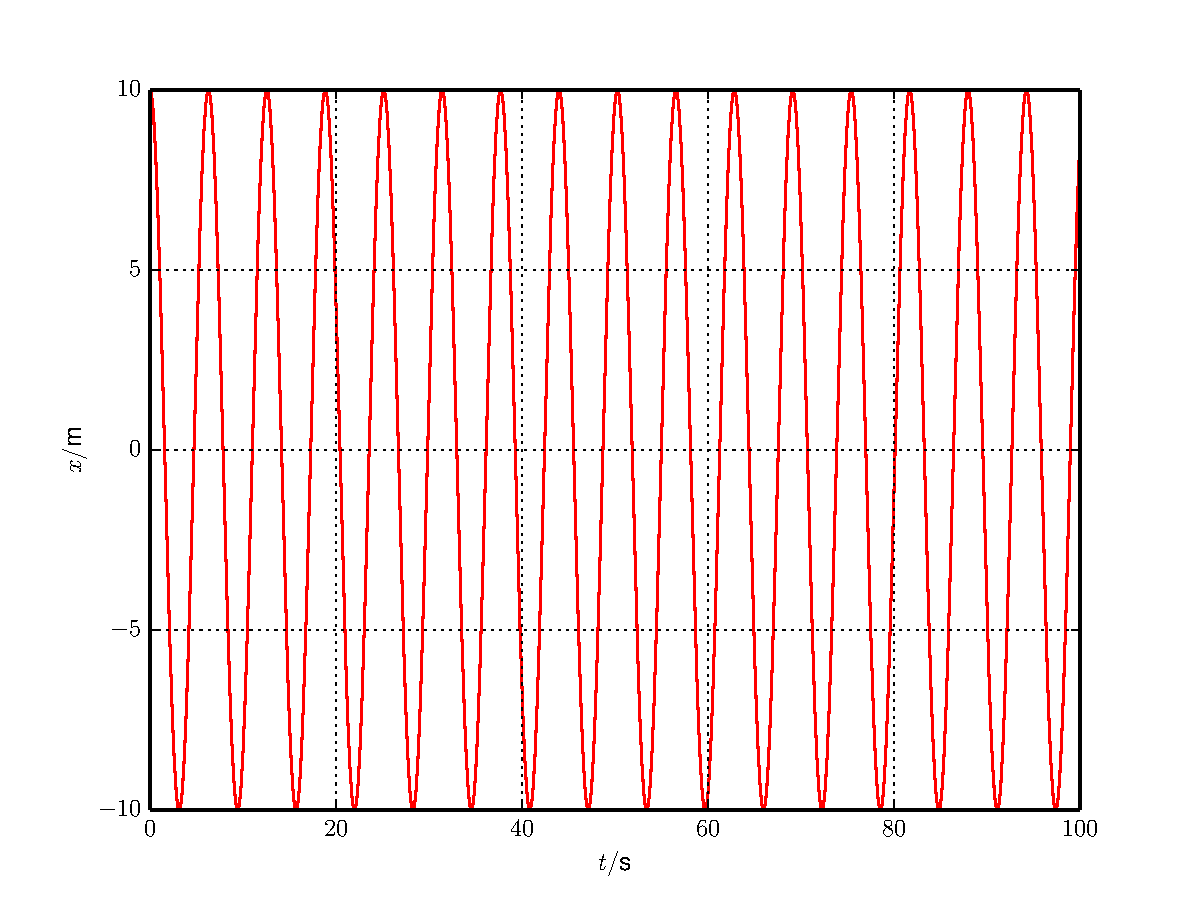
\includegraphics[width = 0.75\textwidth]{../Plots/Plot_2_A_1.pdf}
	\caption{Ergebnis für $x(t)$ für den harmonischen Oszillator.\label{fig:Zentral_X}}
\end{figure}\\
In \cref{fig:Zentral_X} ist die Lösung Dargestellt für $x(t)$, dabei hat sie die Form einer harmonischen Schwingung.\\
\newpage
Als nächstes Wird der Fall betrachtet 
\begin{align}
	\vec{r}_1=10\cdot\vec{e}_x,\ \vec{v}_2=10\cdot\vec{e}_y
\end{align}
\begin{figure}
	\centering
	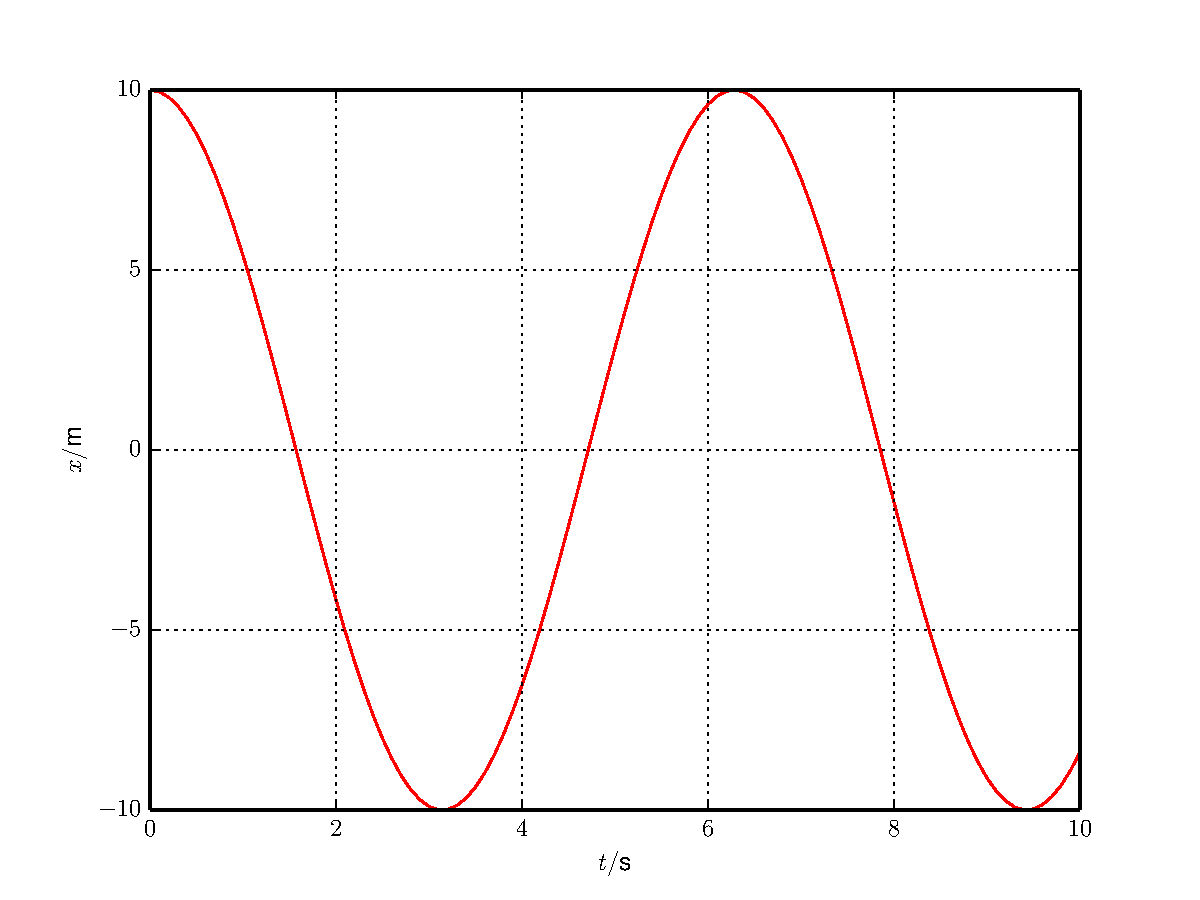
\includegraphics[width = 0.49\textwidth]{../Plots/Plot_2_A_3}
		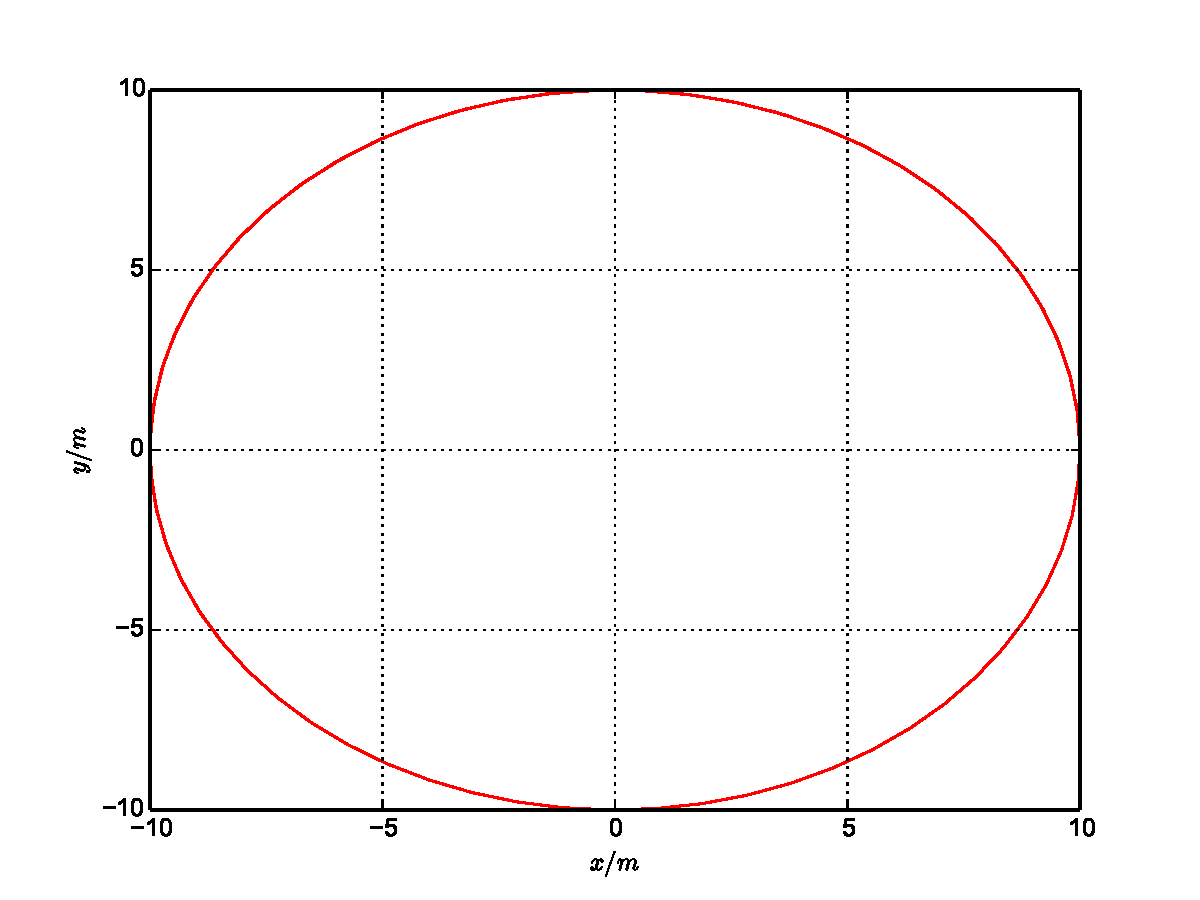
\includegraphics[width = 0.49\textwidth]{../Plots/Plot_2_A_2}
		\caption{Lösung für $x(t)$ und ein mal Lösung für $\vec{r}(t)$, für den Harmonischen Oszillator für $\vec{r}_1$ und $\vec{v}_1$. }
\end{figure}
Es lässt sich erkennen das $x(t)$, wieder eine harmonische Schwingung darstellt und $r(t)$ Ergibt eine harmonische Schwingung um den Koordinaten Uhrsprung.
\newpage
\subsection*{b)}
Hier wird überprüft ob in dem simulierten System erhalten ist.
Dazu wird die Energiedifferenz $\Delta E= |E(t_n)-E(t_{n-1})|$ bestimmt.
Dabei gilt für die Energie
\begin{align}
	E = T + V =& \frac{1}{2}m\left( v^2 - \int \vec{F}(\vec{r} d\vec{r}) \right) =\frac{1}{2}m\left( v^2 + r^2 \right) = \text{const}\\
	\Rightarrow \Delta E =& 0
\end{align}
bestimmt.\\
\begin{figure}
	\centering
	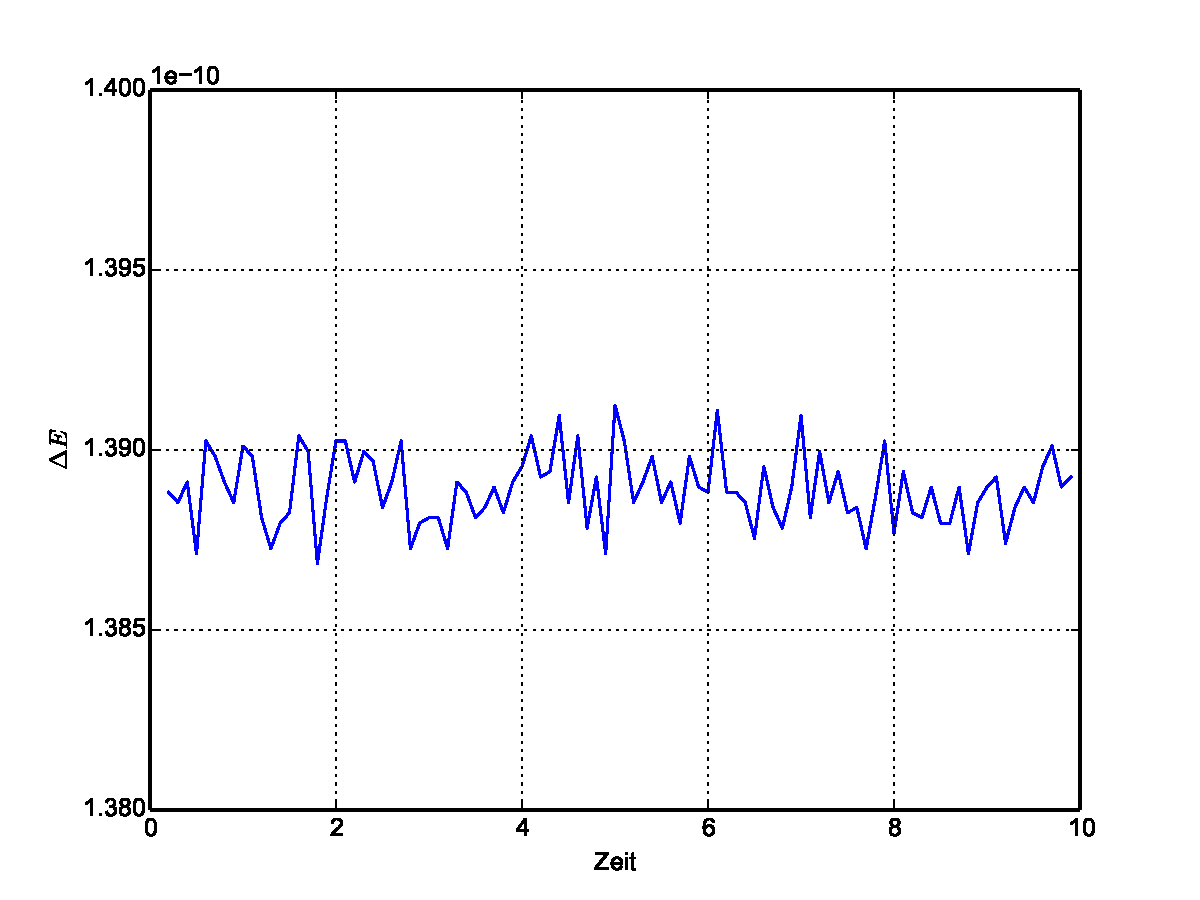
\includegraphics[width = \textwidth]{../Plots/Plot_2_B_Energie.pdf}
	\caption{Die Energie Differenz für verschiedene $t$\label{fig:EnergieDiff}}
\end{figure}
In \cref{fig:EnergieDiff} ist das Ergebnis dargestellt, dabei ist drauf zu achten das $\Delta E$ mit dem Faktor $10^{-10}$ skaliert.
Es gilt demnach $\Delta E\approx 0$